\chapter{First increment}
\label{chap:First Increment}
Test om: Bounce, predefined area
Skal komme væk fra accelerotmeter og gyroscope. 

\section{Requirements}
\label{sec:i1Requirements}
The requirements considered in this increment are marked with blue colouring.

\begin{itemize}
\item The trash bin should catch the trash if the user throws it towards the trash bin and within a predefined area
\begin{itemize}
\item \textcolor{blue}{The robots predefined area should be calculated from the hardware limitations of the motors’ speed}
\end{itemize}
\item The robot should know where it is positioned
\begin{itemize}
\item \textcolor{blue}{The robot should have a starting position, from where it should be able to calculate it's current position}
\item \textcolor{blue}{The robot's starting point should be placed outside its predefined area, such that it moves forward into the area}
\end{itemize}
\item The robot should be able to detect and track the thrown trash
\begin{itemize}
\item \textcolor{blue}{The thrown trash should be detected and tracked by a Microsoft Kinect}
\item The Kinect should send the coordinates of the impact point of the trash to the robot
\end{itemize}
\item The robot should know where the the thrown trash will land
\begin{itemize}
\item \textcolor{blue}{Trajectory prediction should be used to calculate impact point of the thrown trash}
%\item \textcolor{red}{The trajectory prediction should include a bounce prediction}
%\item \textcolor{red}{The bounce-shot should be thrown from a designated side of the camera}
%\item \textcolor{red}{The bounce-shot should bounce into the predefined area where the robot should catch the trash within }
\end{itemize}
\item The robot should be able to move the trash bin, such that the thrown trash lands inside the bin
\begin{itemize}
\item \textcolor{blue}{The robot should be able to turn, drive forward and drive backwards}
\item Multiple trash thrown should not be considered
\end{itemize}
\end{itemize}

These requirements are rudimentary, and the very essence of the project lies within the fulfilment of these requirements. In this increment the fundamentals of the robot’s movement should be implemented, the predefined area should be calculated, a starting point for this area should be determined and the Microsoft Kinect should be able to detect and track an object by using trajectory prediction.

\section{System design}
\label{sec:i1System Design}
The following sections describe how the marked requirements in \ref{sec:i1Requirements} will be attempted to be fulfilled. The theories and ideas behind will be explained subsequently.

\subsection{Predefined area}
\label{sec:i1Predefined area}
The robots predefined area, is an area where the robot should catch the ball within. This area is being made because of the limitations of the robots motors, so the predefined area is where the robot should be expected to catch the ball within.

\subsection{Throwing}
\label{sec:i1Throwing}
The reason why the throw of the object (which in this project will be a table tennis ball) is important, is because the robot should have as much time to move to the collision point as possible. Before the robot moves to the collision point, the Kinect should calculate the where the robot should move, send the data to the robot, and the robot then moves. The Kinect can at any point send new data to the robot, so its course have to be changed, therefore it is important for the robot to have sufficient time to move within the predefined area.    

\subsection{Microsoft Kinect}
\label{sec:i1Microsoft Kinect}
To detect the thrown object, the Kinect has to use one of it's cameras, more specifically the depth sensor in this case. The depth sensor uses a range of infrared speckles, which draw a pattern in the room. Every cluster of speckles can be identified from each other, which makes the kinect able to differentiate between objects in the room. The depth of the specific object can be determined by the use of two cameras, as both cameras can identify the speckles at the object, it can triangulate the distance between the cameras and the object. This speckle pattern technology will only work indoor, and limits the use to only one kinect, as the speckles can be washed out by other lightsources.
\citep{kw}

\subsection{Trajectory prediction}
\label{sec:Trajectory prediction}
When the trash, referred to in this section as the projectile, is detected and the tracking of that projectile has started, the trajectory can be predicted. This prediction is limited to the amount of data sent by the sensory camera, meaning that for every camera reading, one detection of the object is gained. The precision of the prediction will increase according to the time a projectile has been tracked. \newline 
In this project, since the prediction is done indoor, the outdoor weather conditions that might affect the projectile trajectory is not considered. As well, the effects of air resistance, also called drag, will not be considered.

The trajectory of a projectile is the path of a thrown projectile without propulsion, affected by gravity. For calculating a trajectory of a projectile, the initial height, the angle which the projectile is launced from, the speed of the projectile at launch and the gravitational acceleration must be taken into account. \newline 
The initial height in this project is the height at which the projectile is detected, and the angle and speed at which the projectile is launched will be calculated from the first few trackings after detecting the projectile. The gravitational acceleration is considered as \(9.81m/s^2\), which is the standard near the earths surface. \newline
In this project we are interested in catching the projectile, and to do that, we need to calculate the distance the projectile travels before hitting the ground, and the amount of time before the projectile hits the ground. This is done with two mathematical formulas: \newline
\newline 
\begin{math}
g: \ the \ gravitational \ acceleration \ (9.81m/s^2)\newline
\theta: \ the \ angle \ at \ launch 
v: \ the \ speed \ at \ launch\newline
y_{0}: \ the \ initial \ height\newline
d: \ the \ total \ horizontal \ distance \ traveled \ \newline
t: \ the \ time \ of \ flight\newline
v_{vert}: \ the \ vertical \ velocity\newline
v_{hori}: \ the \ horizontal \ velocity\newline
t_{h}: \ the \ time \ since \ first \ detection\newline
d_{t}: \ the \ distance \ at \ time \ t\newline
\end{math}

From these variables we can express the formulas needed to provide the total distance traveled by the projectile, and the amount of time this would take.\newline
The distance traveled is:
\[d = \dfrac{v \ cos \ \theta}{g}(v \ sin \ \theta + \sqrt{(v \ sin \ \theta)^2 \ + \ 2gy_{0}})\] \newline
The time of flight is:
\[t = \dfrac{d}{v \ cos \ \theta} = \dfrac{v \ sin \ \theta \ + \ \sqrt{(v \ sin \ \theta)^2 \ + \ 2gy_{0}}}{g}\]
\newline

To calculate a trajectory of the projectile, the altitude and distance of the projectile at any time during the flight must be calculated, according to the initial height ( \(y_{0}\) ):
\[y = v_{vert}t - \dfrac{1}{2} gt^2\]
\[d_{t} = v_{hori}t\]

After this section, the projectile can be tracked, and the path for a given projectile can be calculated to a certain degree of correctness. 

\subsection{Gyroscope and Accelerometer}
\label{sec:i1Gyroscope and Accelerometer}
For the robot to know where it is positioned. The idea is to use the Lego NXT Gyro sensor, which is a gyroscope and the Lego NXT Accelerometer. 

The purpose of the gyroscope is to get the number of degrees the robot have turned, since the program told the gyroscope to record it. In this way it would be possible to know the heading of the robot, from the start location, which would be at 0 degrees. 

The accelerometer will be used to calculate the distance the robot have traveled since it started moving. The speed of the robot and the time the robot have been at that speed should be recorded, which should be done for every speed change of the robot, to capture the distance it have travled.
(\textcolor{red}{Should look this section over at some point})

\section{Implementation}
\label{sec:i1Implementation}

\subsection{Predefined area}
\label{sec:i1Predefined areaImplementation}
The robots predefined area will be calculated using the travel time of the ball and the speed of the motors used for the project. 
As mentioned in  section \ref{sec:i1ThrowingImplementation}, the bouncing throw would have a travel time of 2 - 2.15 seconds, before landing in the predefined area. The predefined area was calculated using the robot itself. The robot was placed marking its starting point, which will always be its starting point. It was set to turn a specific number of degrees and moving forward, after two seconds the robot would stop. The place the robot stops is marked aswell, which lead to the predefined area seen in figure \ref{figure:Predefined area}. The predefined area have an area of of 2851.5cm\begin{math}^2\end{math} which is 0.285m\begin{math}^2\end{math}.

\begin{figure}[h]
\centering
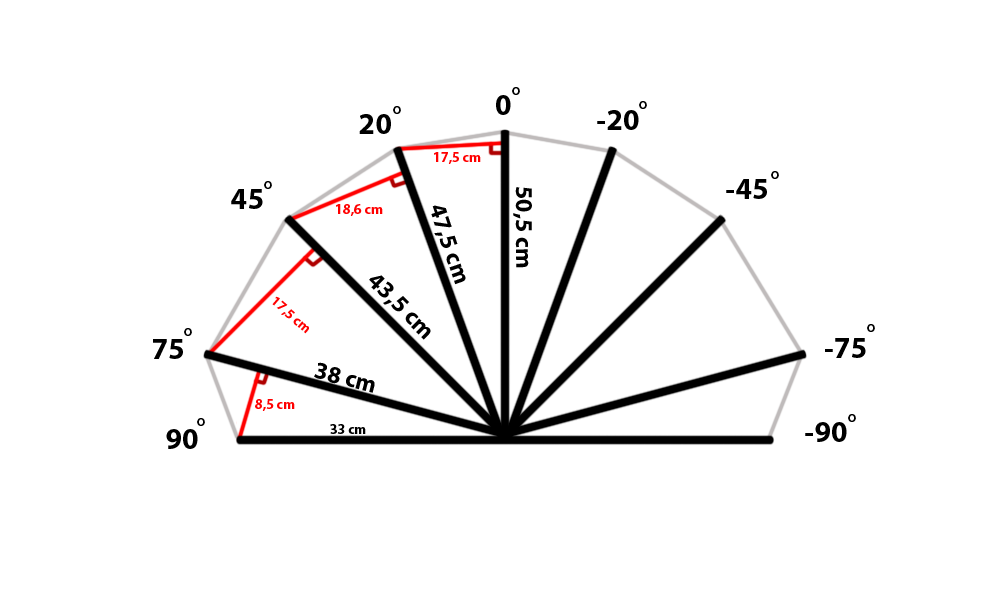
\includegraphics[scale=0.35]{billeder/predefined-area}
\caption{The robots predefined area}
\label{figure:Predefined area}
\end{figure}

\subsection{Throwing}
\label{sec:i1ThrowingImplementation}
Tests have been performed to ensure that the robot is provided the maximum amount of time for calculations and catching the trash. In order to do so, multiple test were conducted, and the results were acquired from a distance of 3 meter, the time it took for the trash (in this case, a table tennis ball) was in average 1.1 second. Multiple tests from a distance of 5 meter were also conducted and that provided an average of 1.25 second. 

With the results from the throwing tests, the group could conclude that a normal throw wouldn't provide enough time for the robot to catch the ball, else the predefined area for the robot had to be very small, due to the limitations of the motors. As mentioned in the \ref{sec:LEGO NXT Servo motor} section, the group calculated the robot's speed to be ~87 RPM, which simply isn't enough to catch trash from a 3 or 5 meter distance. The robot would be able to catch trash within 280mm of itself, given the 1.1 second run time of a 3 meter throw, and therefore nowhere near sufficient enough. 

The group decided after several tests to let the trash (still a table tennis ball) bounce on the floor before it had to be catched, which would give the robot extra time to get to the collision point of the ball. This provided nearly double the amount of time for the throw to be catched, providing an average of 2 seconds from a 3 meter throw and 2.15 seconds from a 5 meter throw.

\subsection{Microsoft Kinect}
\label{sec:i1Microsoft KinectImplementation}

\subsection{Gyroscope and Accelerometer}
\label{sec:i1Gyroscope and AccelerometerImplementation}

\section{Evaluation}
\label{sec:i1Evaluation}
